\documentclass[../result.tex]{subfiles}
\graphicspath{{\subfix{../../../images/}}}
\begin{document}
    The Thermoluminescence Glow curves (TL Glow Curves) obtained using Harshaw TLD Reader 3500 by heating
    the samples from $50^{\circ}C$ to 400◦C at a heating rate of $5^{\circ}C/s$ for both samples after being irradiated with gamma
    rays at 50 Gy and 100Gy are shown here:

    \FloatBarrier\begin{multicols}{2}
        \begin{Figure}
            \centering
            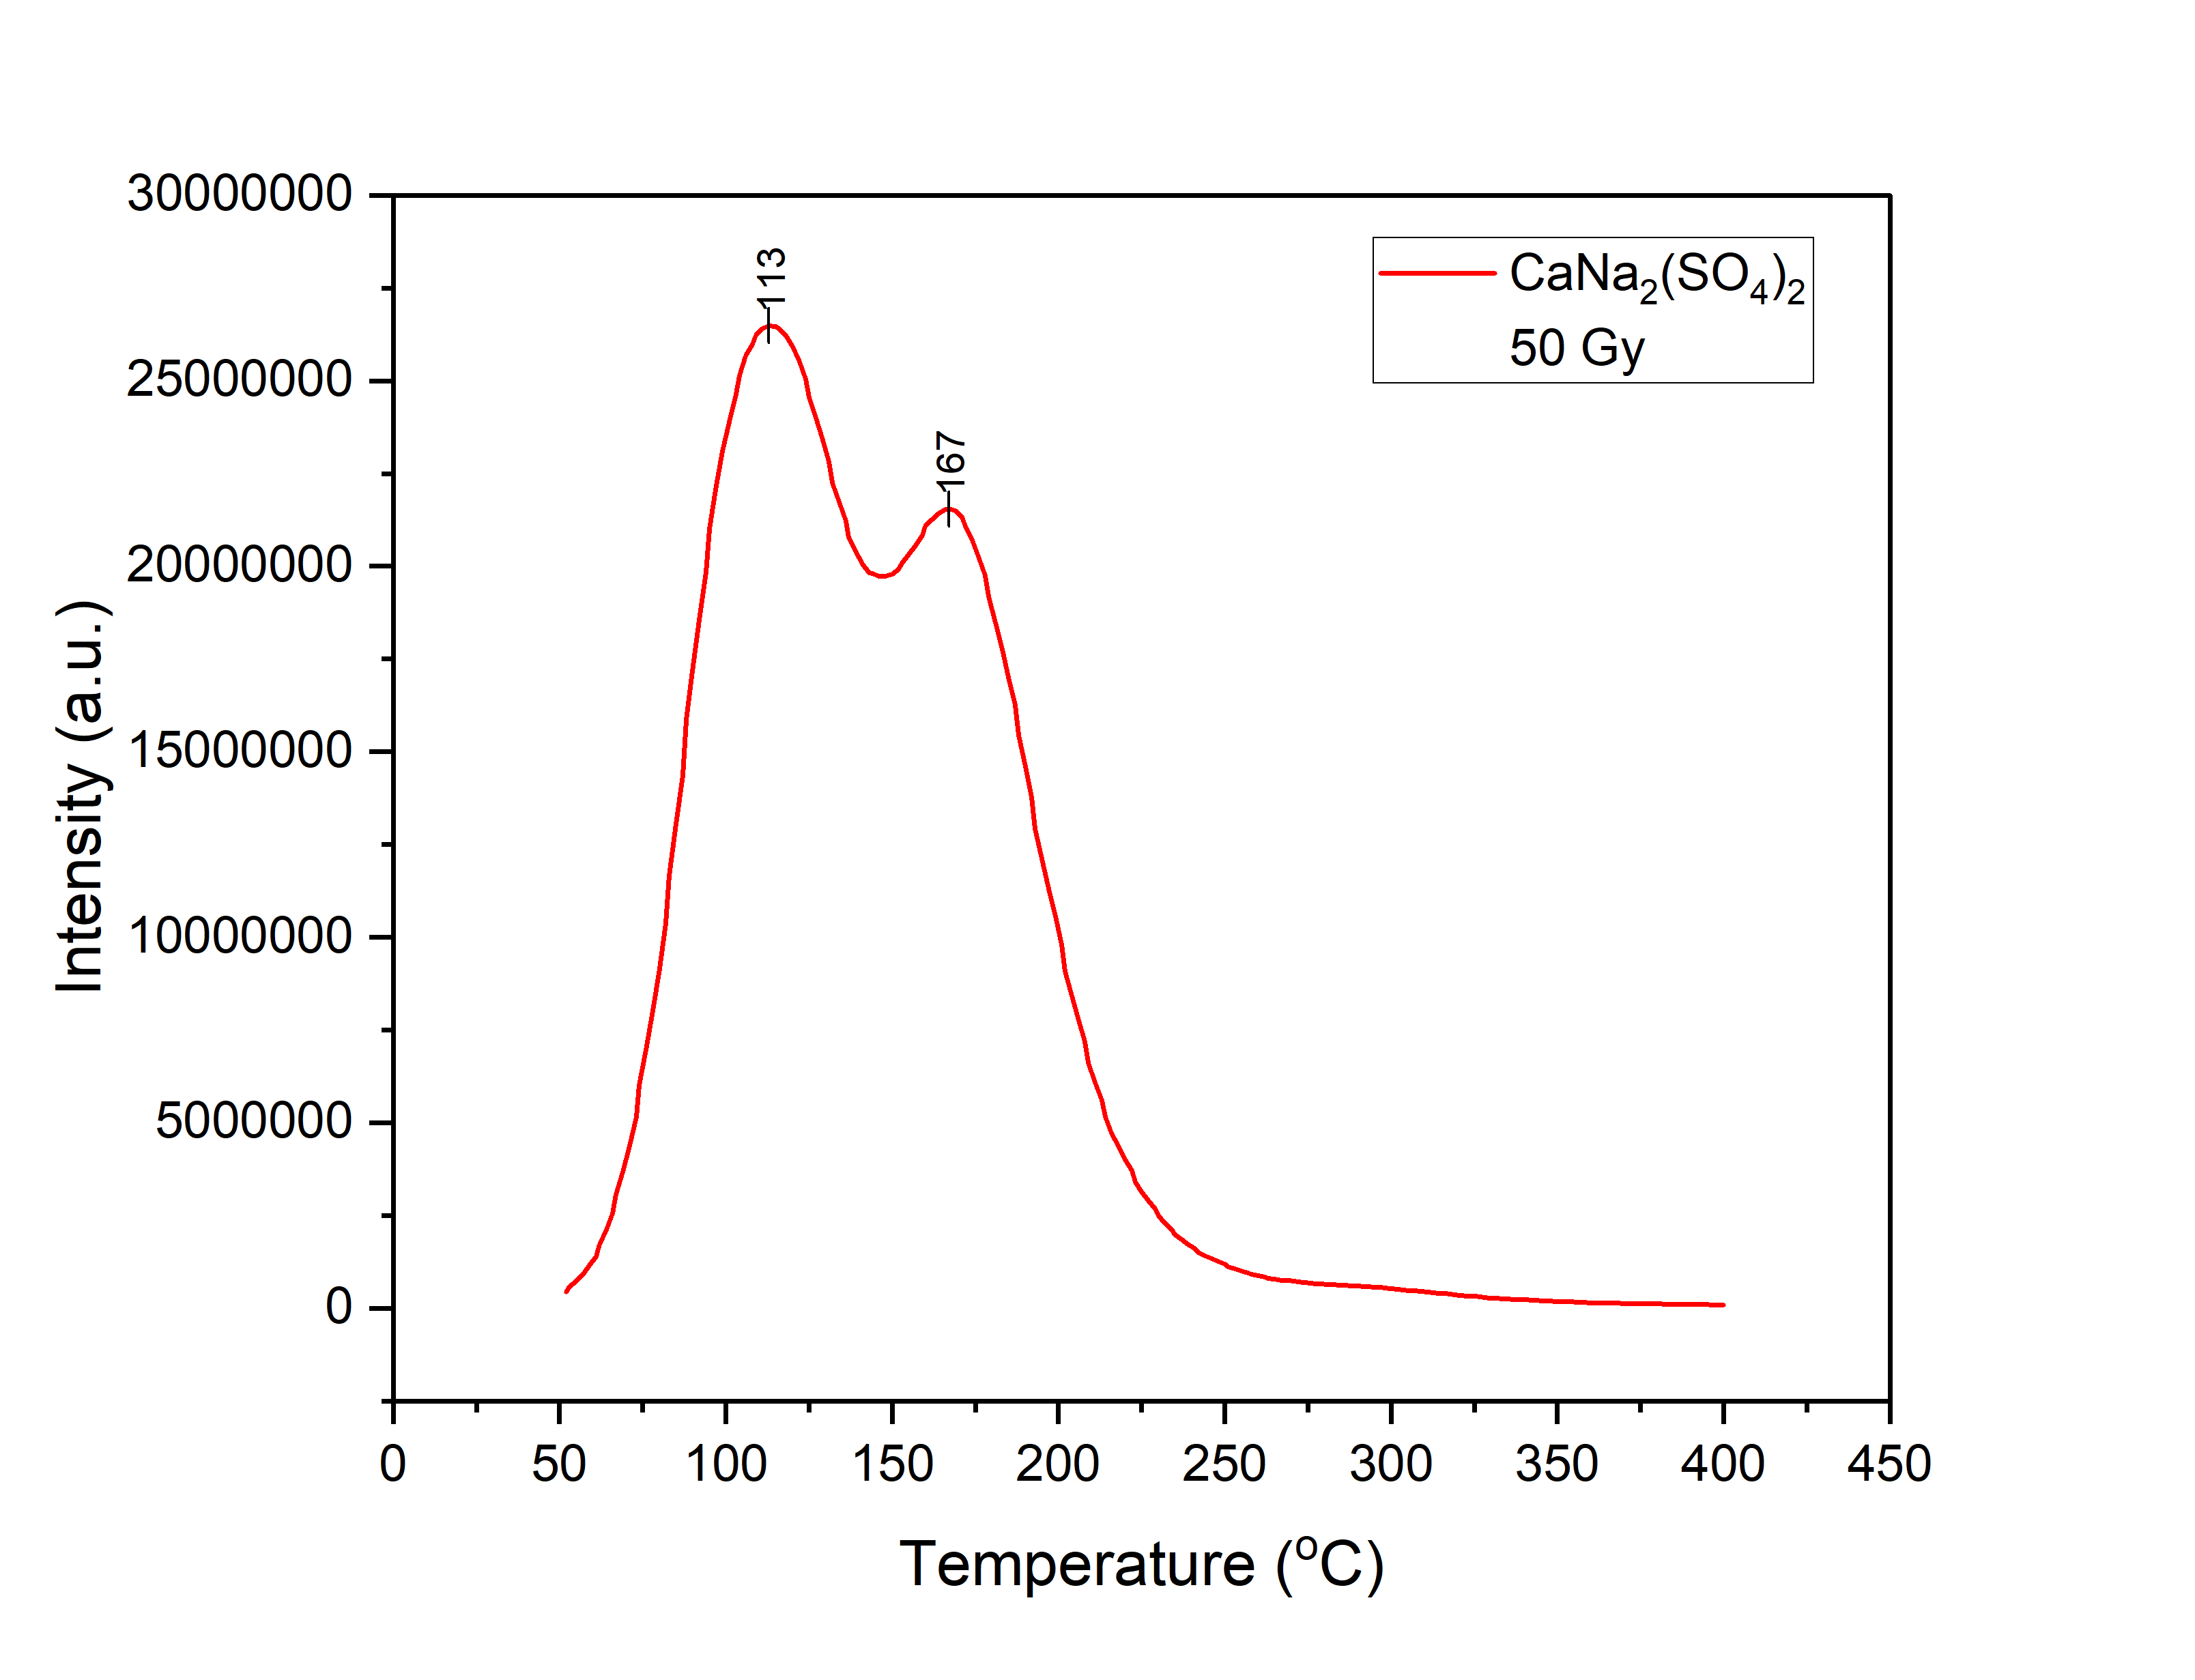
\includegraphics[width=\linewidth]{Cana50Gy.png}
            \captionof{figure}{Dose response for Calcium Sodium Sulphate when irradiated with Gamma ray at 50 
            Gy}\label{fig:Cana50Gy}
        \end{Figure}
        \begin{Figure}
            \centering
            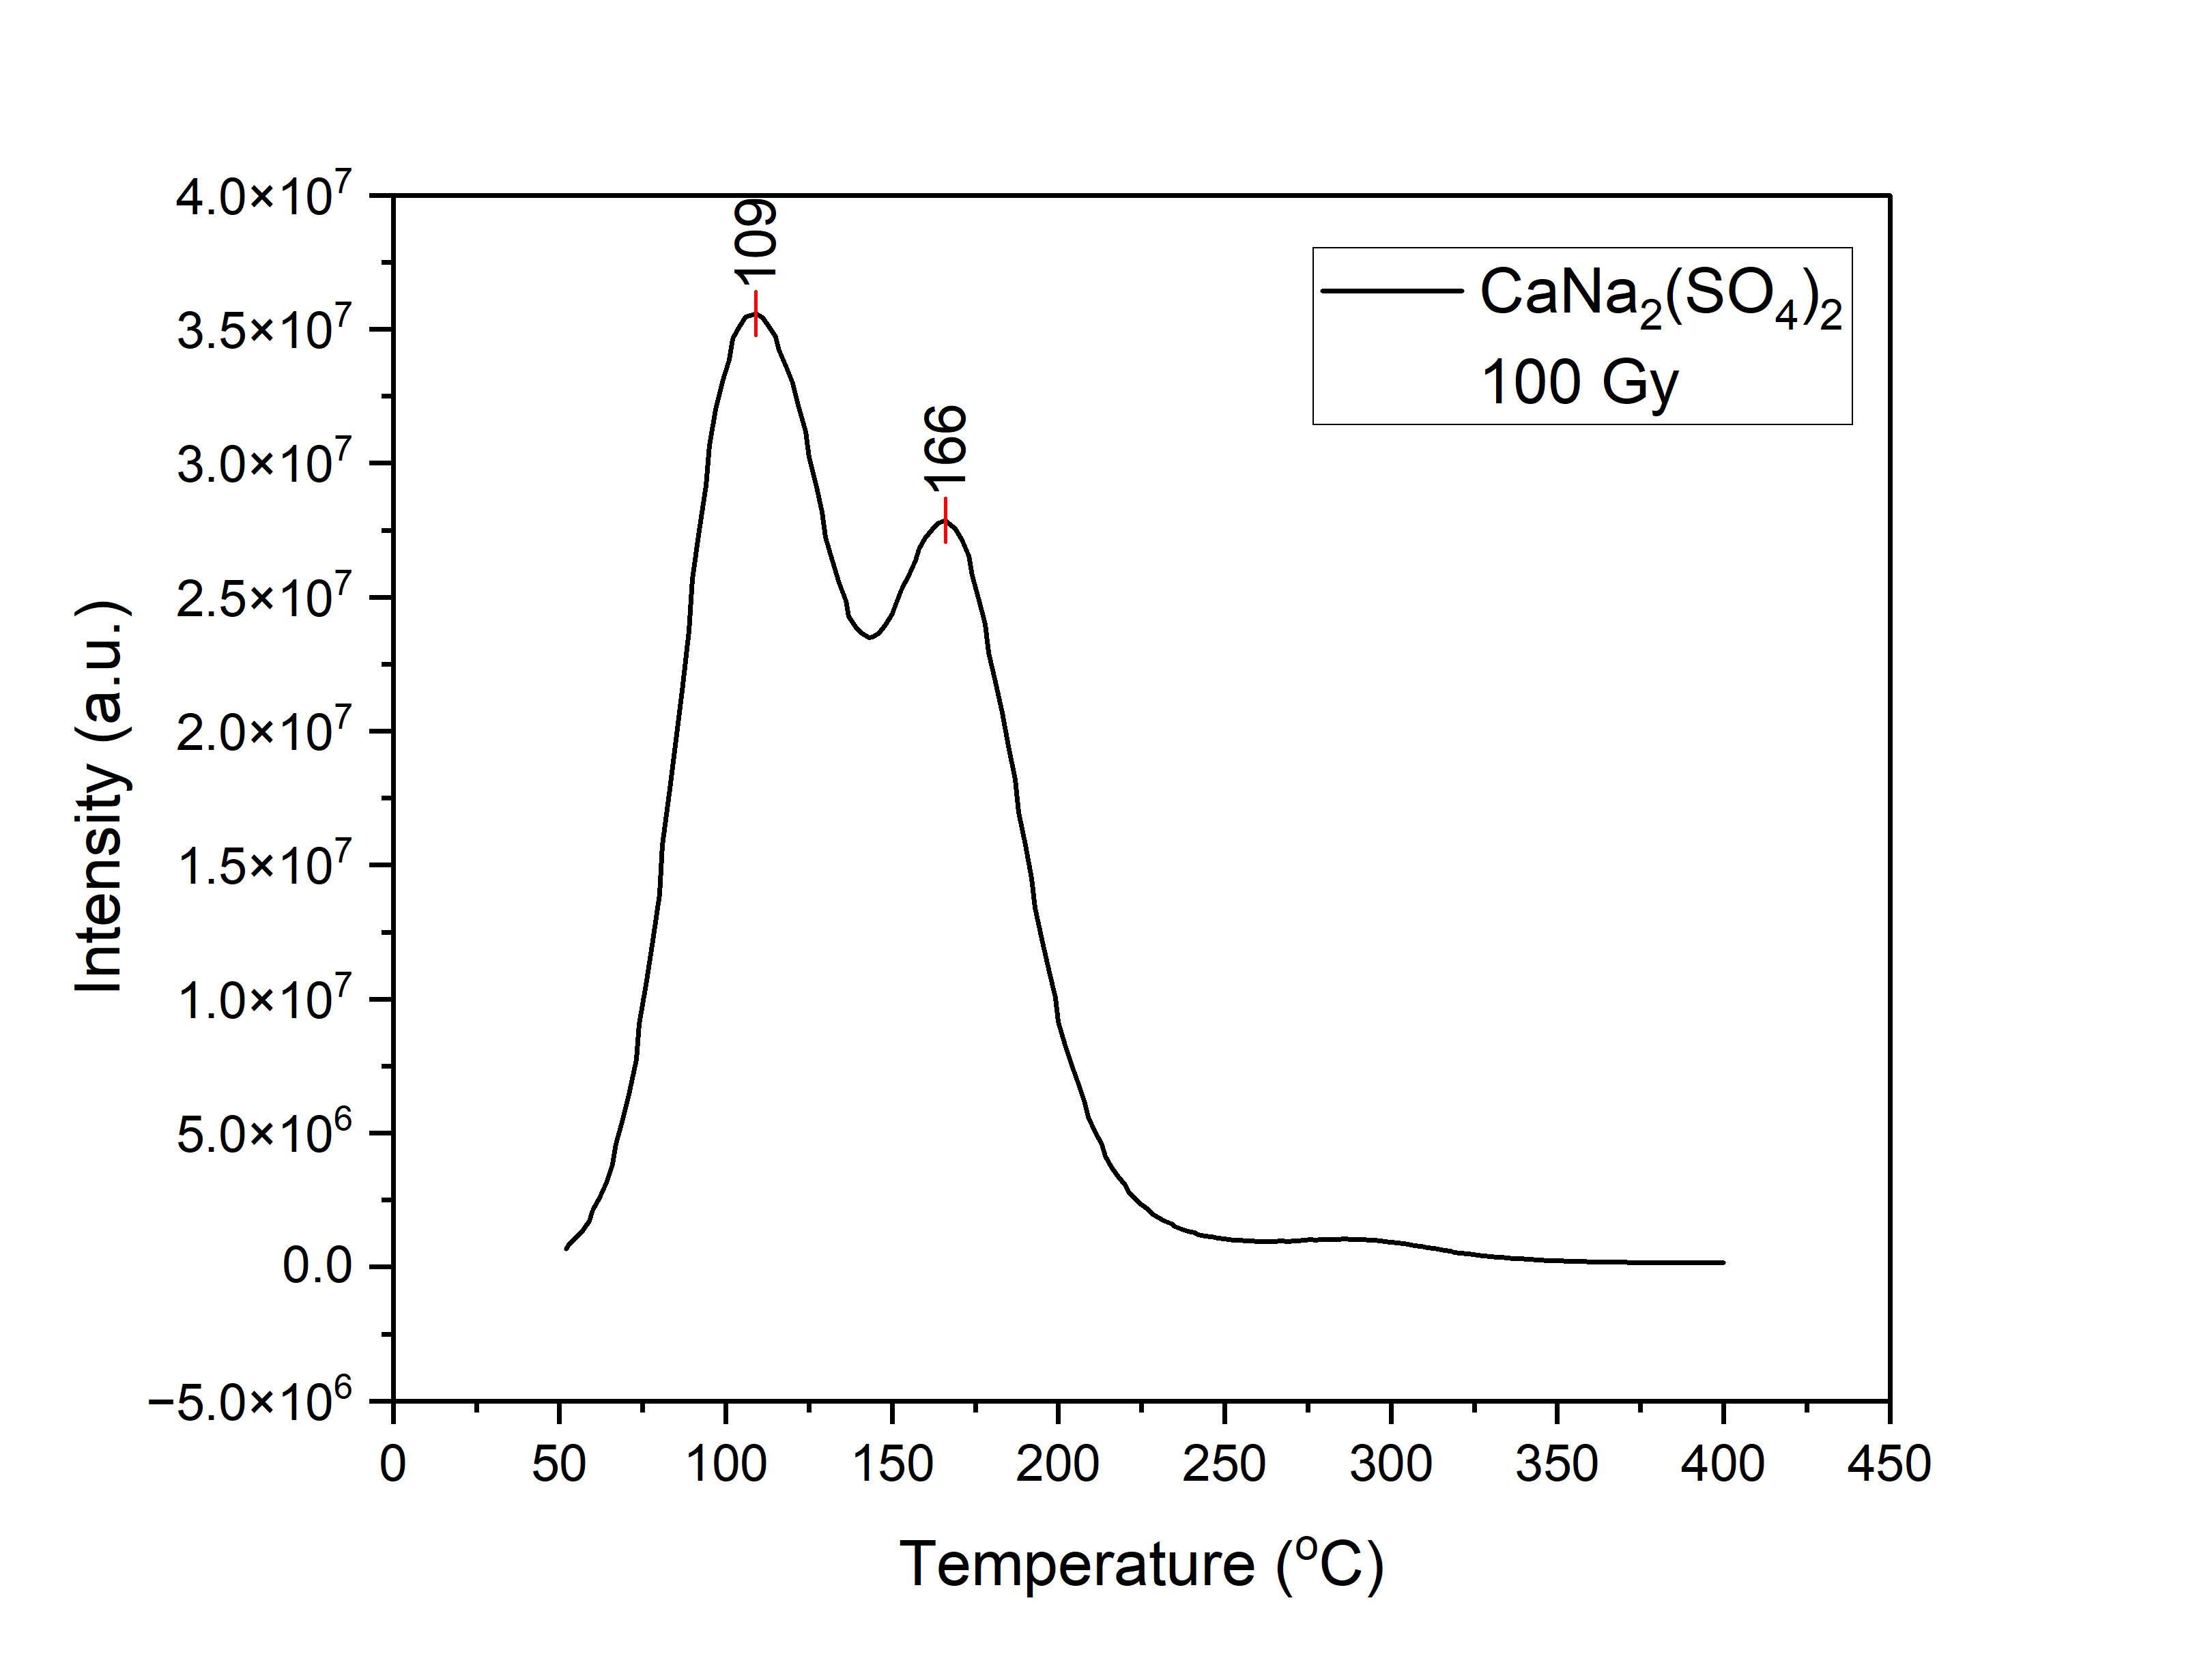
\includegraphics[width=\linewidth]{Cana100Gy.png}
            \captionof{figure}{Dose response for Calcium Sodium Sulphate when irradiated with Gamma ray at 100 
            Gy}\label{fig:Cana100Gy}
        \end{Figure}
        \begin{Figure}
            \centering
            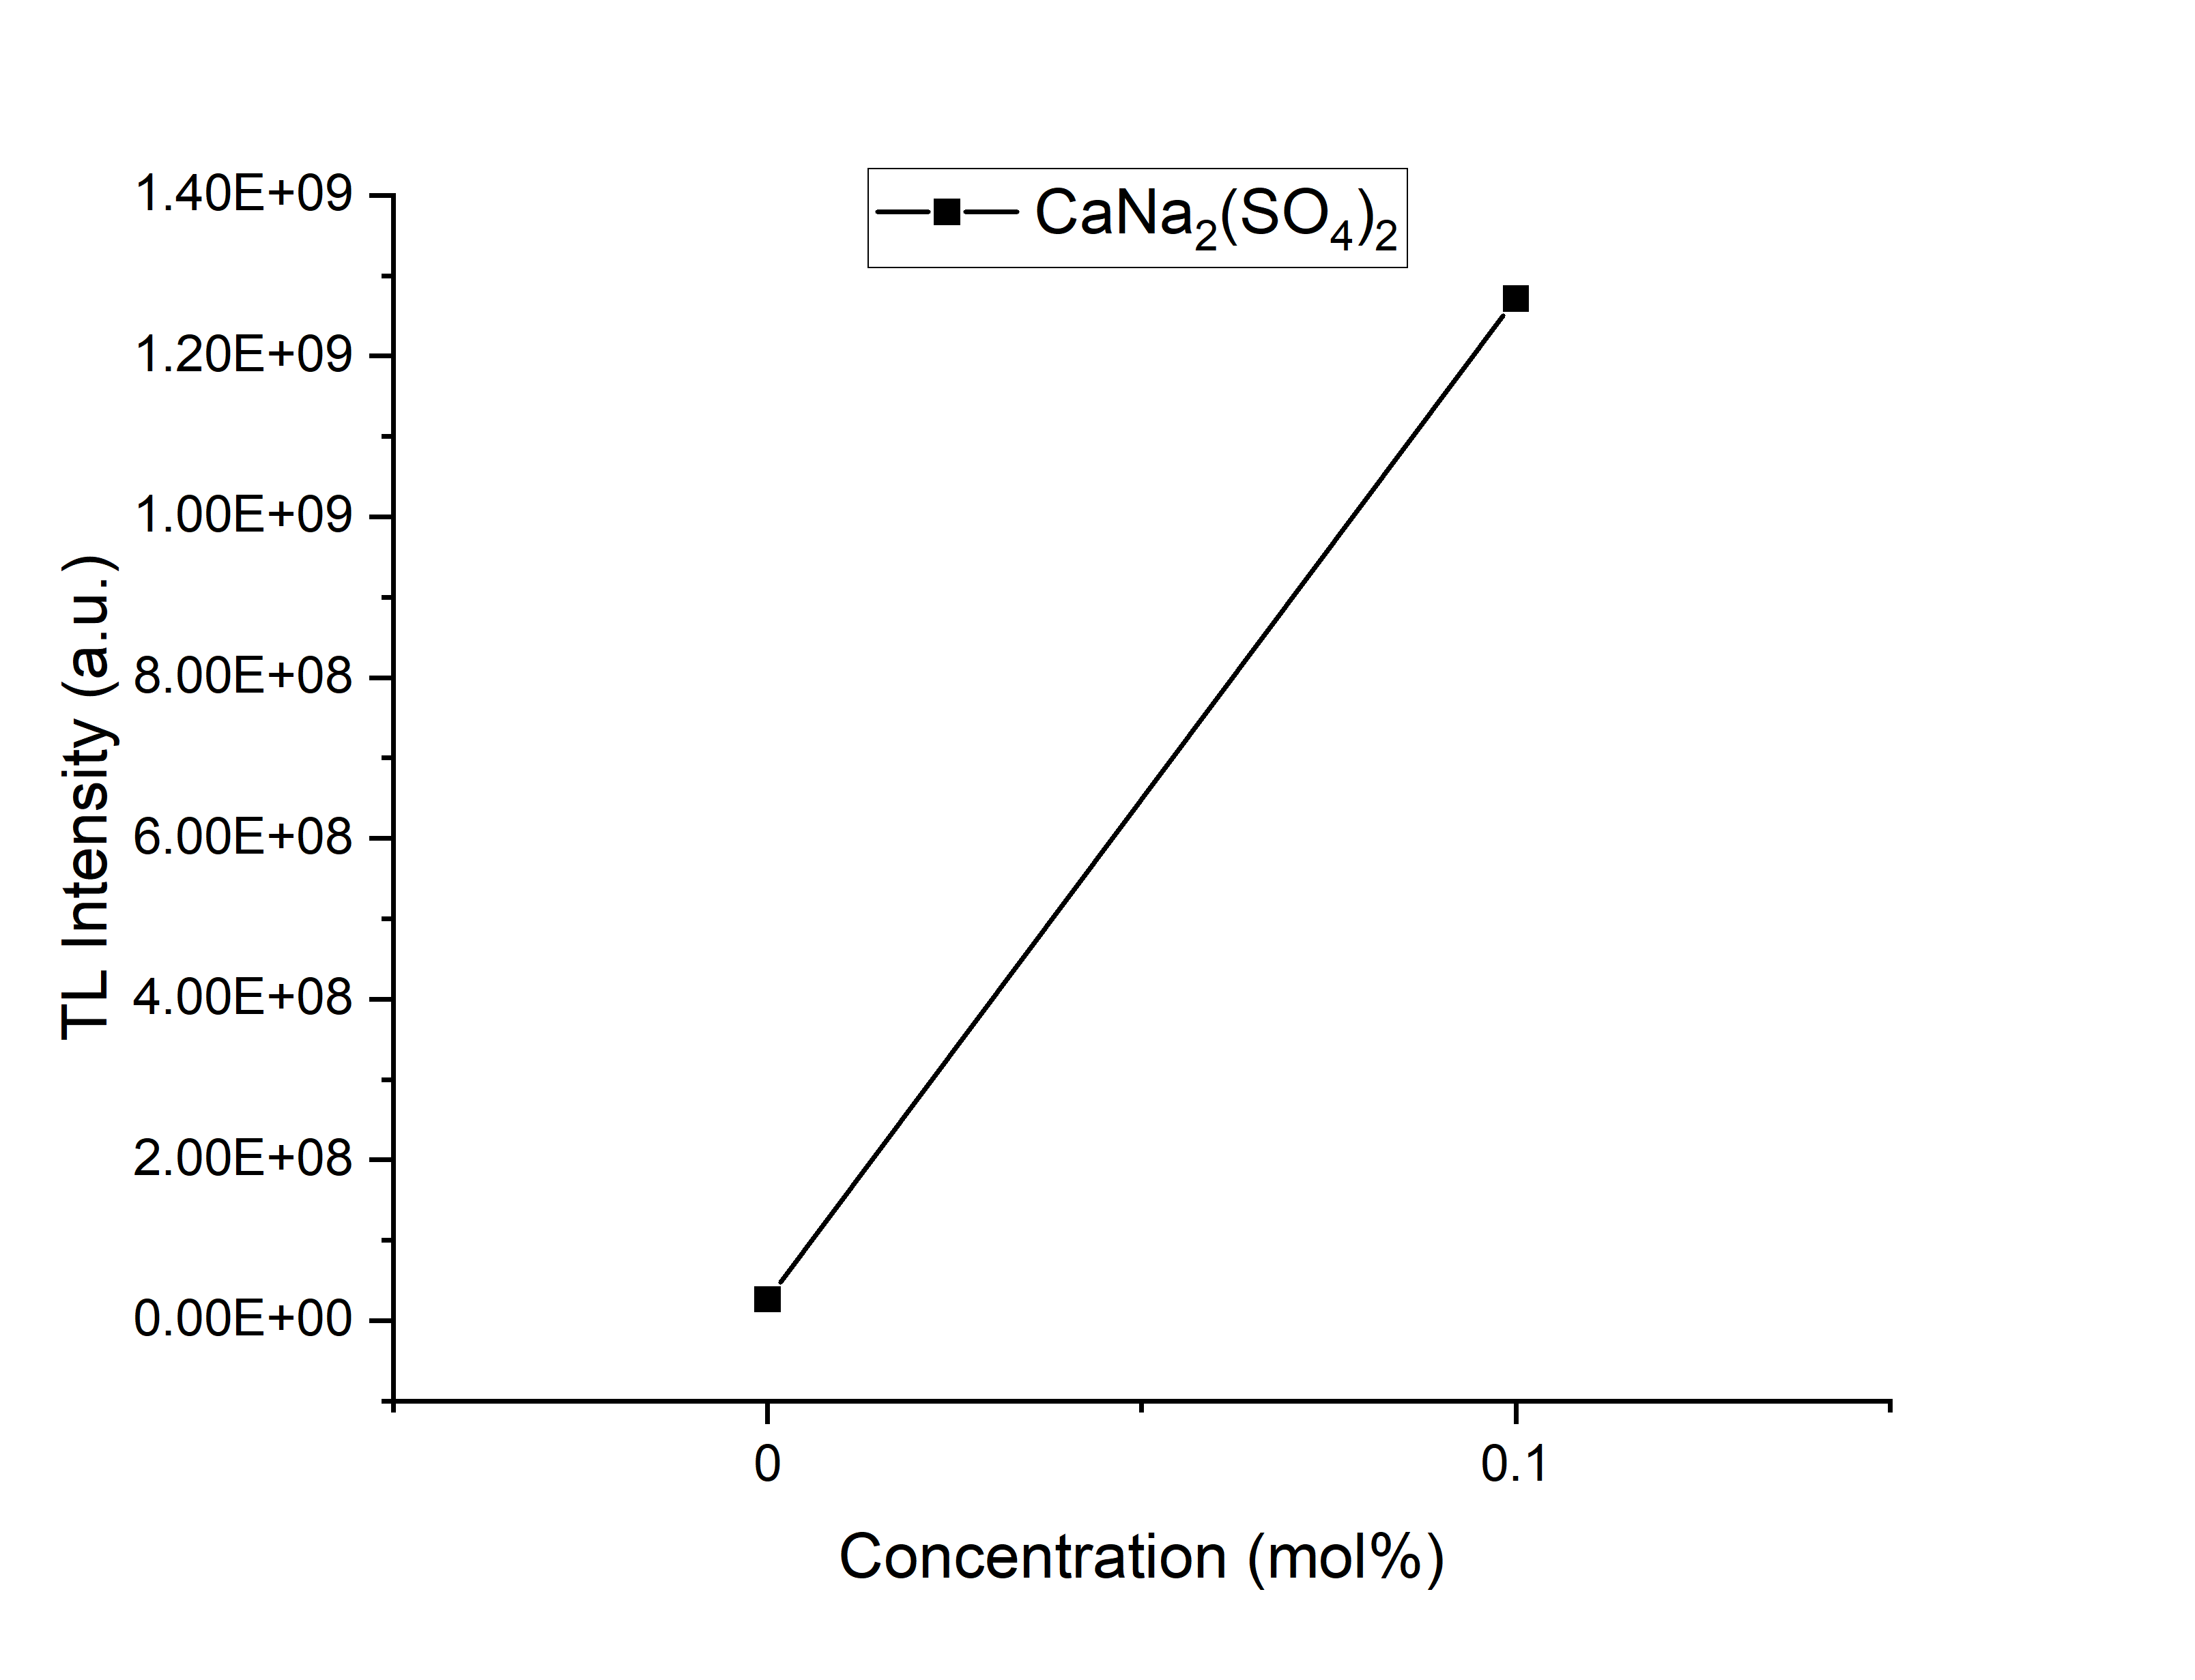
\includegraphics[width=\linewidth]{Canacompare.png}
            \captionof{figure}{Effect of doping on dose response of Calcium Sodium Sulphate}\label{fig:Canacompare}
        \end{Figure}
        \begin{Figure}
            \centering
            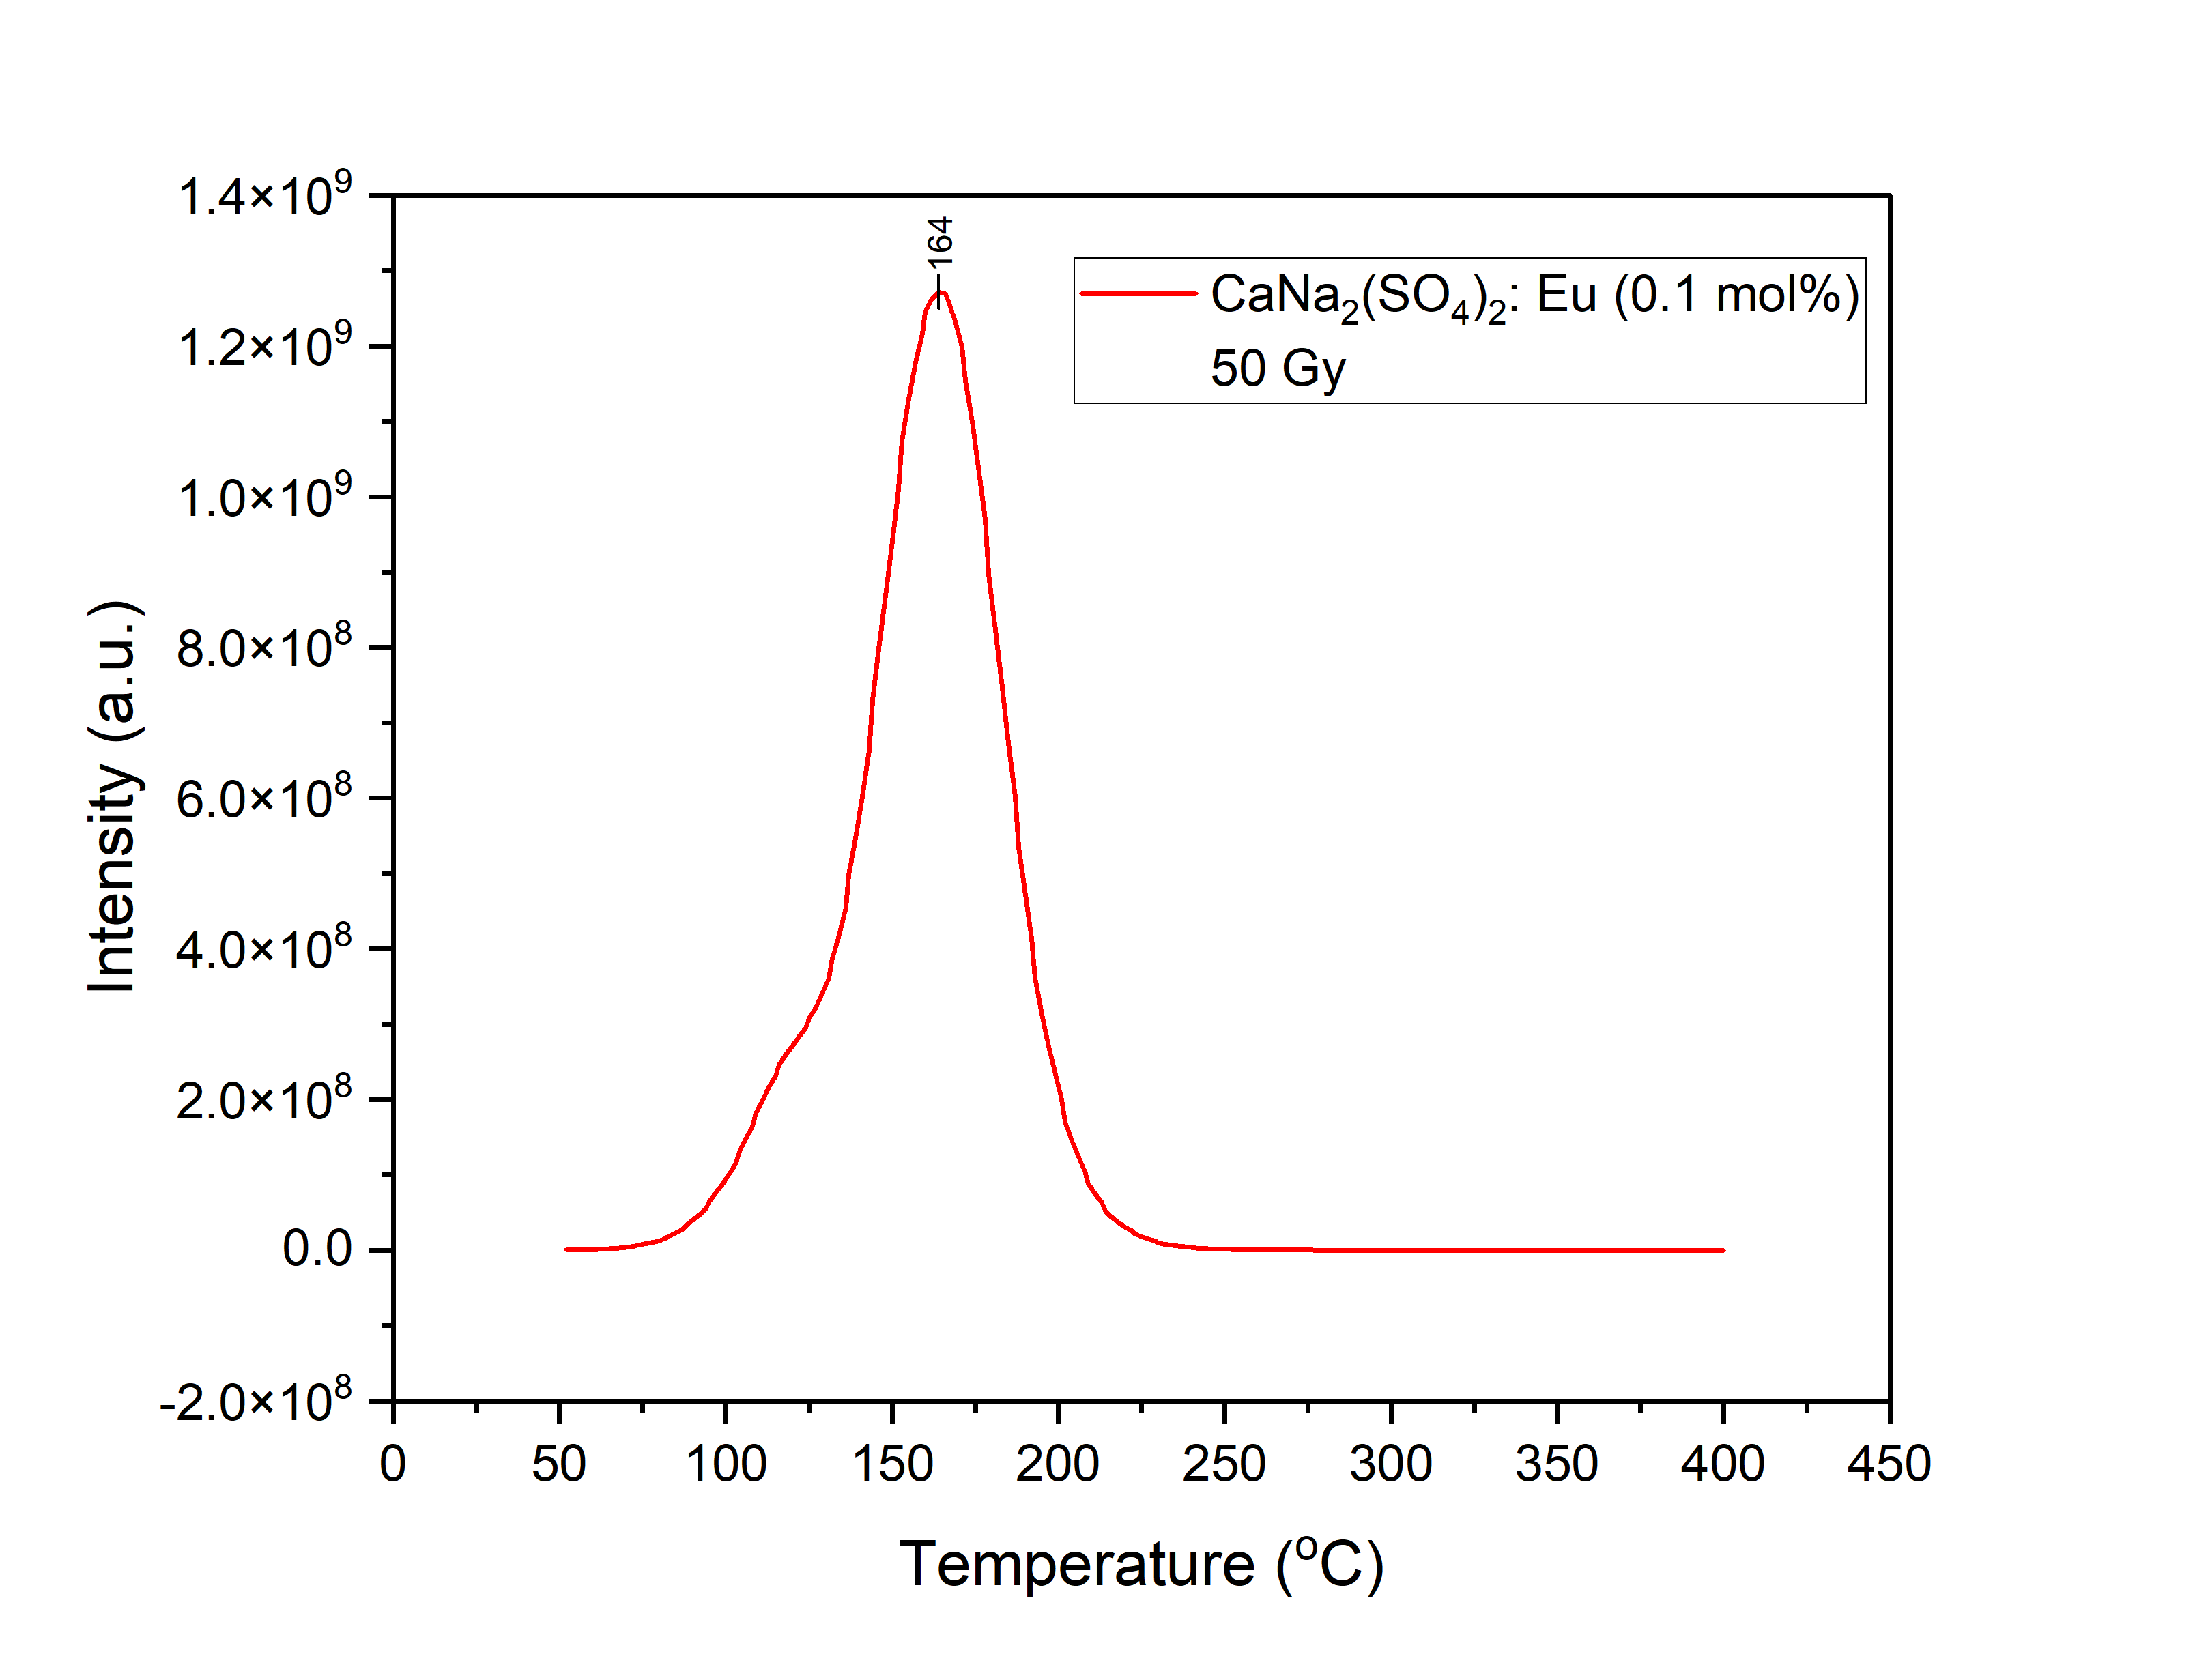
\includegraphics[width=\linewidth]{CaEu50.png}
            \captionof{figure}{Dose response for Calcium Sodium Sulphate after doping with Europium when 
            irradiated with Gamma ray at 50 Gy}\label{fig:CaEu50}
        \end{Figure}
    \end{multicols}

    Another study that we undertook is comparison of intensity of TL with the concentration of dopant. As
    can be seen, with addition of dopant, the glow curves come close to having a single peak as compared to pure
    sample. Also the thermoluminescence intensity for doped sample is more compared to that of the pure sample.
    However, conclusive evidence cannot be provided as only one concentration of doped sample was synthesized
    and further analysis is required.
\end{document}